\documentclass{article}
\usepackage{fancyhdr} % Required for custom headers
\usepackage{lastpage} % Required to determine the last page for the footer
\usepackage{extramarks} % Required for headers and footers
\usepackage[usenames,dvipsnames]{color} % Required for custom colors
\usepackage{graphicx} % Required to insert images
\usepackage{listings} % Required for insertion of code
\usepackage{courier} % Required for the courier font
\usepackage{lipsum} % Used for inserting dummy 'Lorem ipsum' text into the template
\usepackage{caption}
\usepackage{subcaption}
\usepackage{amsmath}
\usepackage{amsfonts}
\usepackage{amssymb}
\usepackage{epstopdf}
\usepackage{placeins}
\usepackage{color} 
\usepackage{fancyvrb} 
\usepackage{setspace}
\usepackage[numbered]{bookmark}
\usepackage{tikz}
\usepackage{pgfplots}
\usetikzlibrary{calc}
\usetikzlibrary{pgfplots.fillbetween, backgrounds}
\usetikzlibrary{positioning}
\usetikzlibrary{arrows}
\usetikzlibrary{pgfplots.groupplots}
\usetikzlibrary{arrows.meta}
\usetikzlibrary{plotmarks}
\usetikzlibrary{calc}

\usepgfplotslibrary{groupplots}
\pgfplotsset{compat=newest} 
%\pgfplotsset{plot coordinates/math parser=false}
\DeclareGraphicsExtensions{.pdf,.png,.jpg}
\graphicspath{{figs/}}


\DeclareMathOperator{\E}{\mathbb{E}}


\newcommand{\Conv}{\mathop{\scalebox{1.5}{\raisebox{-0.2ex}{$\ast$}}}}%

% Margins
\topmargin=-0.45in
\evensidemargin=0in
\oddsidemargin=0in
\textwidth=6.5in
\textheight=9.0in
\headsep=0.25in

\linespread{1.2} % Line spacing

% Set up the header and footer
\pagestyle{fancy}
\lhead{\hmwkAuthorName} % Top left header
\chead{\hmwkTitle} % Top center head
\rhead{\hmwkClass} % Top right header
\lfoot{} % Bottom left footer
\cfoot{} % Bottom center footer
\rfoot{Page\ \thepage\ of\ \protect\pageref{LastPage}} % Bottom right footer
\renewcommand\headrulewidth{0.4pt} % Size of the header rule
\renewcommand\footrulewidth{0.4pt} % Size of the footer rule

%\setlength\parindent{0pt} % Removes all indentation from paragraphs
\definecolor{MyDarkGreen}{rgb}{0.0,0.4,0.0} % This is the color used for comments
\lstloadlanguages{Perl} % Load Perl syntax for listings, for a list of other languages supported see: ftp://ftp.tex.ac.uk/tex-archive/macros/latex/contrib/listings/listings.pdf
\lstset{language=Perl, % Use Perl in this example
        frame=single, % Single frame around code
        basicstyle=\small\ttfamily, % Use small true type font
        keywordstyle=[1]\color{Blue}\bf, % Perl functions bold and blue
        keywordstyle=[2]\color{Purple}, % Perl function arguments purple
        keywordstyle=[3]\color{Blue}\underbar, % Custom functions underlined and blue
        identifierstyle=, % Nothing special about identifiers                                         
        commentstyle=\usefont{T1}{pcr}{m}{sl}\color{MyDarkGreen}\small, % Comments small dark green courier font
        stringstyle=\color{Purple}, % Strings are purple
        showstringspaces=false, % Don't put marks in string spaces
        tabsize=5, % 5 spaces per tab
        %
        % Put standard Perl functions not included in the default language here
        morekeywords={rand},
        %
        % Put Perl function parameters here
        morekeywords=[2]{on, off, interp},
        %
        % Put user defined functions here
        morekeywords=[3]{test},
       	%
        morecomment=[l][\color{Blue}]{...}, % Line continuation (...) like blue comment
        numbers=left, % Line numbers on left
        firstnumber=1, % Line numbers start with line 1
        numberstyle=\tiny\color{Blue}, % Line numbers are blue and small
        stepnumber=5 % Line numbers go in steps of 5
}

% Creates a new command to include a perl script, the first parameter is the filename of the script (without .pl), the second parameter is the caption
\newcommand{\perlscript}[2]{
\begin{itemize}
\item[]\lstinputlisting[caption=#2,label=#1]{#1.pl}
\end{itemize}
}

% Header and footer for when a page split occurs within a problem environment
\newcommand{\enterProblemHeader}[1]{
\nobreak\extramarks{#1}{#1 continued on next page\ldots}\nobreak
\nobreak\extramarks{#1 (continued)}{#1 continued on next page\ldots}\nobreak
}

% Header and footer for when a page split occurs between problem environments
\newcommand{\exitProblemHeader}[1]{
\nobreak\extramarks{#1 (continued)}{#1 continued on next page\ldots}\nobreak
\nobreak\extramarks{#1}{}\nobreak
}

\setcounter{secnumdepth}{0} % Removes default section numbers
\newcounter{homeworkProblemCounter} % Creates a counter to keep track of the number of problems

\newcommand{\homeworkProblemName}{}
\newenvironment{homeworkProblem}[1][Problem \arabic{homeworkProblemCounter}]{ % Makes a new environment called homeworkProblem which takes 1 argument (custom name) but the default is "Problem #"
\stepcounter{homeworkProblemCounter} % Increase counter for number of problems
\renewcommand{\homeworkProblemName}{#1} % Assign \homeworkProblemName the name of the problem
\section{\homeworkProblemName} % Make a section in the document with the custom problem count
\enterProblemHeader{\homeworkProblemName} % Header and footer within the environment
}{
\exitProblemHeader{\homeworkProblemName} % Header and footer after the environment
}

\newcommand{\problemAnswer}[1]{ % Defines the problem answer command with the content as the only argument
\noindent\framebox[\columnwidth][c]{\begin{minipage}{0.98\columnwidth}#1\end{minipage}} % Makes the box around the problem answer and puts the content inside
}

\newcommand{\homeworkSectionName}{}
\newenvironment{homeworkSection}[1]{ % New environment for sections within homework problems, takes 1 argument - the name of the section
\renewcommand{\homeworkSectionName}{#1} % Assign \homeworkSectionName to the name of the section from the environment argument
\subsection{\homeworkSectionName} % Make a subsection with the custom name of the subsection
\enterProblemHeader{\homeworkProblemName\ [\homeworkSectionName]} % Header and footer within the environment
}{
\enterProblemHeader{\homeworkProblemName} % Header and footer after the environment
}

%----------------------------------------------------------------------------------------
%	NAME AND CLASS SECTION
%----------------------------------------------------------------------------------------
%%%%%%%%%%%%%%%%%%%%%%%%%%%%%%%%%%%%%%%%%%%%%%%%%%%%%%%%%%%%%%%%%%%%%%%%%%%%%%%%%%%%%%%%%
\newcommand{\hmwkTitle}{Homework \#01} % Assignment title
\newcommand{\hmwkDueDate}{\today} % Due date
\newcommand{\hmwkClass}{EE 264 (Summer 2017)} % Course/class
\newcommand{\hmwkAuthorName}{Solutions} % Your name
%%%%%%%%%%%%%%%%%%%%%%%%%%%%%%%%%%%%%%%%%%%%%%%%%%%%%%%%%%%%%%%%%%%%%%%%%%%%%%%%%%%%%%%%%
%----------------------------------------------------------------------------------------
%	TITLE PAGE
%----------------------------------------------------------------------------------------
\title{
\vspace{2in}
\textmd{\textbf{\hmwkClass:\ \hmwkTitle}}\\
\normalsize\vspace{0.1in}\small{Due\ on\ \hmwkDueDate}\\
\vspace{0.1in}\large{\textit{\hmwkClassInstructor\ \hmwkClassTime}}
\vspace{3in}
}

\author{\textbf{\hmwkAuthorName}}
\date{} % Insert date here if you want it to appear below your name

%----------------------------------------------------------------------------------------

\begin{document}
\section{Problem 1}
\subsection{(i) $y[n] = x[n] - 0.5x[n-1] + 0.5x[n-2]$}
\subsubsection{(a)}
By applying the linearity and time shift properties of the $z$-transform:
\begin{align} \nonumber
Y(z) &= X(z)(1 - 0.5z^{-1} + 0.5z^{-2}) \\
H(z) &= \frac{Y(z)}{X(z)} = 1 - 0.5z^{-1} + 0.5z^{-2} \\
			H(z) &= \frac{z^2 - 0.5z + 0.5}{z^2}
\end{align}
\subsubsection{(b)}
From the derivation above we can see that $H(z)$ has two poles at the origin ($p_1 = p_2 = 0$). We can use the function \texttt{roots([1, -1, 0.5])} to determine that $H(z)$ has two zeros $z_1 = 0.5 + j0.5$ and $z_1^* = 0.5 - j0.5$. Note that since the polynomial coefficients are real, complex roots appear in complex conjugate pairs.

We can determine that this system is causal by inspecting the difference equation and noticing that at any given time $n$, the output only depends on the current and past samples $\{x[n], x[n-1], x[n-2]\}$. 

As the system is causal, the ROC is the exterior of a circle whose radius is the magnitude of the outermost pole. In this case, we only have poles at the origin. Hence, the ROC is the entire $z$-plan with the exception of $z = 0$. Hence, $\mathrm{ROC} = \mathbb{C}^*$.

Since the ROC contains the unit circle, this system is stable.

\begin{center}
	\resizebox{0.5\linewidth}{!}{\input{figs/hw01q1b_pole-zero1.tex}}
\end{center}
	
\subsubsection{(c)}
\texttt{>> freqz([1, -0.5, 0.5], 1)}

Note that the Matlab uses the coefficients of polynomials of $z^{-1}$.

\begin{figure}[h!]
	\centering
	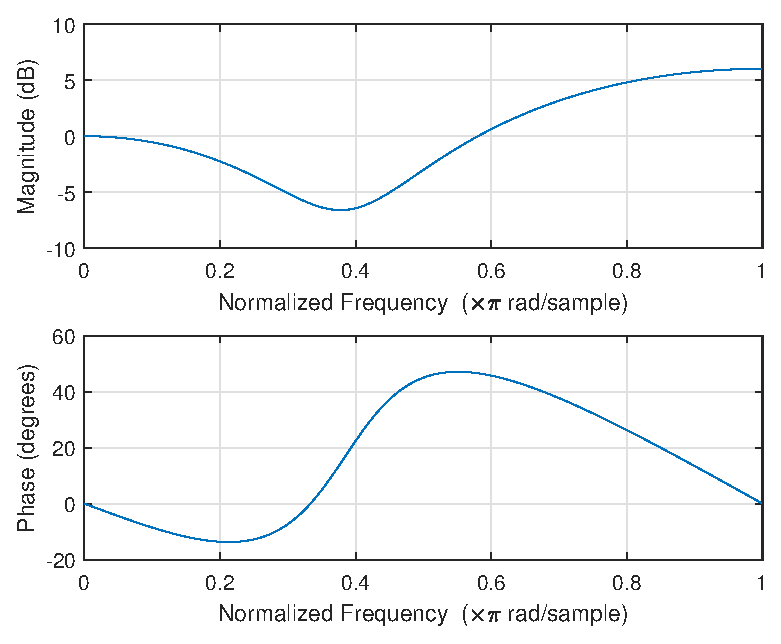
\includegraphics[scale=0.7]{figs/hw01q1c_freqz1.eps}
	\caption{Maginute and phase response for the system defined by the difference equation (i).}
\end{figure}

\subsection{(ii) $y[n] - 0.5y[n-1] + 0.2y[n-2] + 0.3y[n-3] = x[n] + 0.5x[n-1] + 0.1x[n-2] + 0.5x[n-3]$}

\subsubsection{(a)}
By applying the linearity and time shift properties of the $z$-transform:
\begin{align} \nonumber
Y(z)(1 -0.5z^{-1} + 0.2z^{-2} + 0.3z^{-3}) &= X(z)(1 + 0.5z^{-1} + 0.1z^{-2} + 0.5z^{-3}) \\
H(z) &= \frac{Y(z)}{X(z)} = \frac{1 + 0.5z^{-1} + 0.1z^{-2} + 0.5z^{-3}}{1 -0.5z^{-1} + 0.2z^{-2} + 0.3z^{-3}} \\
H(z) &= \frac{z^3 + 0.5z^{2} + 0.1z + 0.5}{z^3 -0.5z^{2} + 0.2z + 0.3}
\end{align}
\subsubsection{(b)}
\noindent For the zeros: \\
\texttt{roots([1, 0.5, 0.1, 0.5])}\\
This results in $z_1 = 0.9494$, $z_2 = 0.2247 + j0.69$, $z_3 = z_2^* = 0.2247 -j0.69$.

\noindent For the poles:\\
\texttt{roots([1, -0.5, 0.2, 0.3])}\\
This results in $z_1 = 0.9494$, $z_2 = 0.2247 + j0.69$, $z_3 = z_2^* = 0.2247 -j0.69$.

This system is also causal, since, from the difference equation, at any given time $n$, the output only depends on the current and past samples. In this case, the outermost poles are the complex conjugate pair with $|p_2| = 0.8043$. Therefore, $\mathrm{ROC} = \{|z| > 0.8043\}$.

The ROC contains the unit circle, therefore this system is stable.

\begin{center}
	\resizebox{0.5\linewidth}{!}{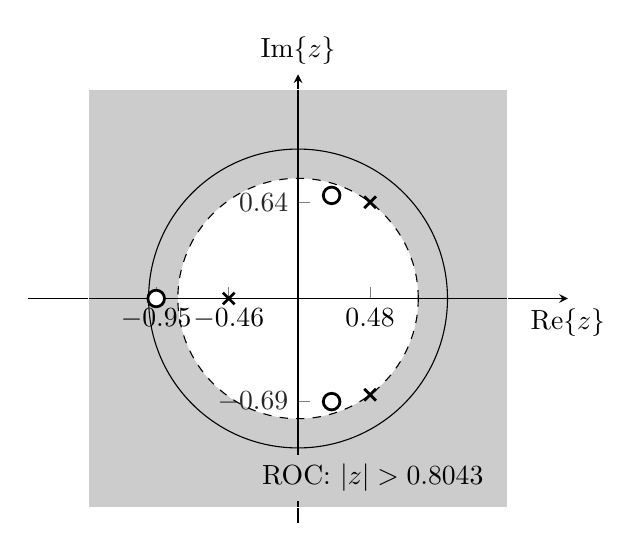
\begin{tikzpicture} 
\begin{axis}[
axis equal,
axis lines*=middle,
enlargelimits = false,
xmax=1.5,
xmin=-1.5,
ymin=-1.5,
ymax=1.5,
axis line style={->,>=stealth},
xlabel={$\mathrm{Re}\{z\}$},
ylabel={$\mathrm{Im}\{z\}$},
every axis x label/.style={
    at={(ticklabel* cs:1)},
    anchor=north,
},
every axis y label/.style={
    at={(ticklabel* cs:1)},
    anchor=south,
},
xtick={-0.9494, -0.4637, 0.4819},
ytick={0.644, -0.6900},
xticklabel style = {xshift=0cm},
every outer y axis line/.append style={white!15!black},
every y tick label/.append style={font=\color{white!15!black}},
legend style={draw=white!15!black,fill=white,legend cell align=left}]
\addplot[line width=1pt,mark=*, only marks, mark size = 3pt, mark options={fill=white}] coordinates {(-0.9494, 0) (0.2247, 0.6900) (0.2247, -0.6900)};
\addplot[line width=1pt,mark=x, only marks, mark size = 3pt] coordinates {   (0.4819, 0.644) (0.4819, -0.644) (-0.4637, 0)};
\draw (axis cs:0,0) circle [black, line width=2pt, radius=1];

\draw[name path=A, dashed] (axis cs:0,0) circle [black, line width=2pt, radius=0.8043];
\draw [name path=B, white] (axis cs:-1.4, -1.4) rectangle (axis cs:1.4,1.4);
\addplot [
thick,
color=black,
fill=black, 
fill opacity=0.2
]
fill between[
of=A and B,
];
\node[fill=black!20] (roc) at (axis cs:0.5, -1.2) {ROC: $|z| > 0.8043$};
\end{axis}
\end{tikzpicture}
}
\end{center}

\subsubsection{(c)}
\texttt{>> freqz([1, 0.5, 0.1, 0.5], [1, -0.5, 0.2, 0.3])}

\begin{figure}[h!]
	\centering
	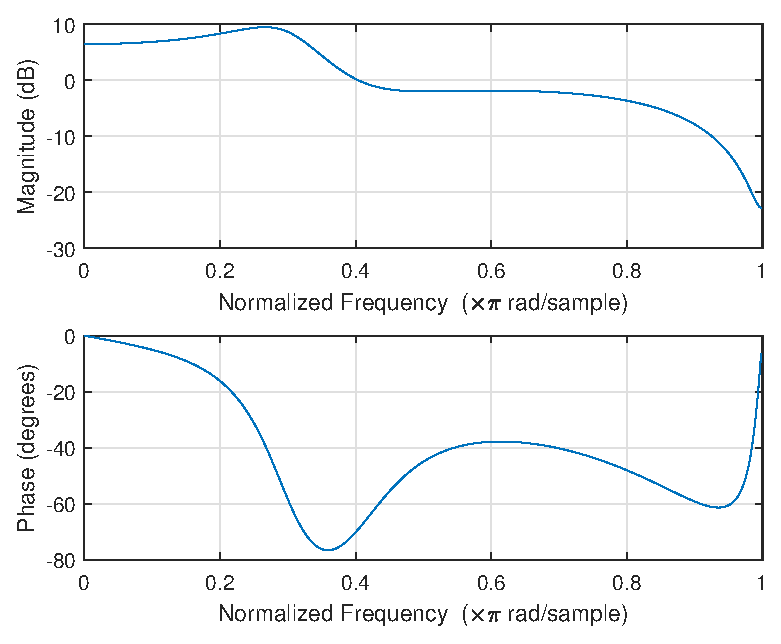
\includegraphics[scale=0.7]{figs/hw01q1c_freqz2.eps}
	\caption{Maginute and phase response for the system defined by the difference equation (ii).}
\end{figure}

\subsection{(d)}

By inspecting the magnitude plots of both systems, we see that while system (i) has a gain of $-6.4$ dB at $\omega =0.4\pi$, system (ii) has a gain of 0 dB at the same frequency. Therefore, system (ii) will produce the output with highest amplitude when the input is $x[n] = \cos(0.4\pi n)$.
	
\section{Problem 2: Echo cancellation}
\subsection{(a)}
For the first echo generating system:
\begin{align} \nonumber
Y(z) &= X(z) + \alpha X(z)z^{-N}
H_1(z) = \frac{Y(z)}{X(z)} = 1 + \alpha z^{-N}
\end{align}

For the second echo generating system:
\begin{align} \nonumber
Y(z) &= X(z) + \alpha Y(z)z^{-N}
H_2(z) = \frac{Y(z)}{X(z)} = \frac{1}{1 - \alpha z^{-N}}
\end{align}

From the problem statement, the first echo is delayed by 0.1 s. Since the sampling frequency is 8 kHz, this corresponds to 
\begin{equation}
N = T_{echo}f_s = 0.1\cdot 8\times 10^3 = 800
\end{equation}

\subsection{(b)}
The code to generate these plots is included at the end of the solutions to this question.

\begin{figure}[h!]
	\centering
	\begin{subfigure}[h!]{0.5\textwidth}
		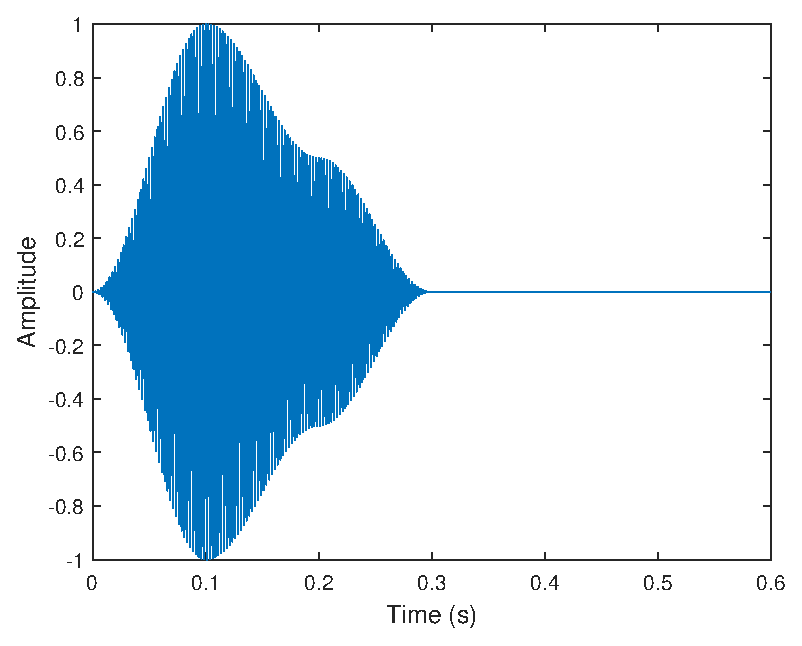
\includegraphics[width=\textwidth]{figs/hw01q2_echoed1.eps}
		\caption{Echo-generating system 1}
	\end{subfigure}%
	~ %add desired spacing between images, e. g. ~, \quad, \qquad etc.
	%(or a blank line to force the subfigure onto a new line)
	\begin{subfigure}[h!]{0.5\textwidth}
		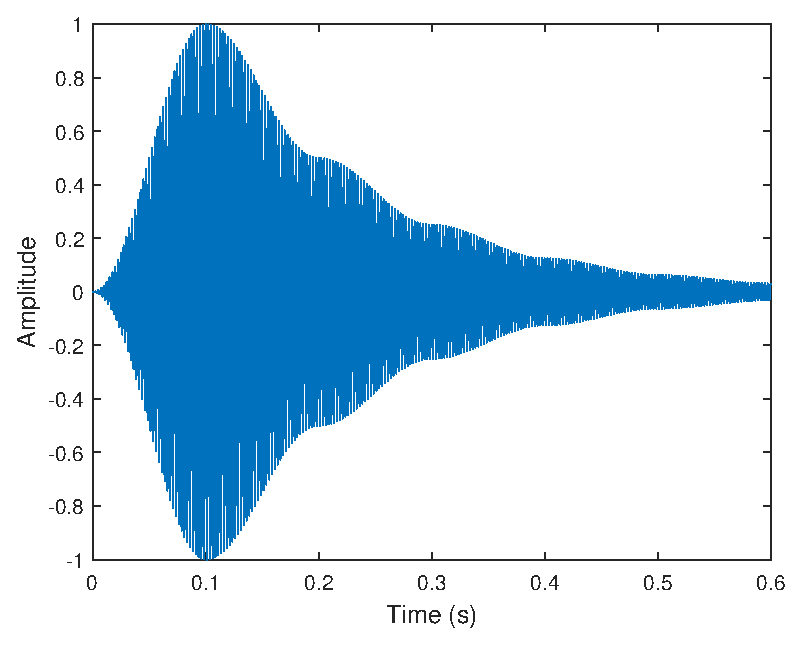
\includegraphics[width=\textwidth]{figs/hw01q2_echoed2.eps}
		\caption{Echo-generating system 2}
	\end{subfigure}
	\caption{Waveforms of the echoed signals generated by the echo-generating systems (a) 1 and (b) 2.}
\end{figure}

\subsection{(c)}

For each system, we just need to calculate its inverse:
\begin{align}
G_1(z) &= H_1^{-1}(z) = \frac{1}{1 + \alpha z^{-N}} \tag{system 1} \\
G_2(z) &= H_2^{-1}(z) = 1 - \alpha z^{-N} \tag{system 2}
\end{align}

System 1 is IIR, as it has poles different from zero. System 2 is FIR, as all its poles are at zero. 

Note that while system 2 is always stable, system 1 is only stable if $|\alpha| < 1$. 

\subsection{(d)}

We clearly see from the images below that perfect echo cancellation was achieved for both systems. System 1 could fail only if $|\alpha| \geq 1$, in which case, the system could become unstable.

\begin{figure}[h!]
	\centering
	\begin{subfigure}[h!]{0.5\textwidth}
		\includegraphics[width=\textwidth]{figs/hw01q2_echoed_rec1.eps}
		\caption{Echo cancellation 1}
	\end{subfigure}%
	~ %add desired spacing between images, e. g. ~, \quad, \qquad etc.
	%(or a blank line to force the subfigure onto a new line)
	\begin{subfigure}[h!]{0.5\textwidth}
		\includegraphics[width=\textwidth]{figs/hw01q2_echoed_rec2.eps}
		\caption{Echo cancellation 2}
	\end{subfigure}
	\caption{Recovered waveforms after echoed cancellation of echoed signals produced by the echo-generating systems (a) 1 and (b) 2.}
\end{figure}

\subsection{Code for problem 2}
% This file was automatically created from the m-file 
% "m2tex.m" written by USL. 
% The fontencoding in this file is UTF-8. 
%  
% You will need to include the following two packages in 
% your LaTeX-Main-File. 
%  
% \usepackage{color} 
% \usepackage{fancyvrb} 
%  
% It is advised to use the following option for Inputenc 
% \usepackage[utf8]{inputenc} 
%  
  
% definition of matlab colors: 
\definecolor{mblue}{rgb}{0,0,1} 
\definecolor{mgreen}{rgb}{0.13333,0.5451,0.13333} 
\definecolor{mred}{rgb}{0.62745,0.12549,0.94118} 
\definecolor{mgrey}{rgb}{0.5,0.5,0.5} 
\definecolor{mdarkgrey}{rgb}{0.25,0.25,0.25} 
  
\DefineShortVerb[fontfamily=courier,fontseries=m]{\$} 
\DefineShortVerb[fontfamily=courier,fontseries=b]{\#} 
  
\noindent                                                                      
 \hspace*{-1.6em}{\scriptsize 1}$  $\color{mgrey}#%% Template for the echo cancelling problem#\color{black}$$\\
 \hspace*{-1.6em}{\scriptsize 2}$  clear, $\color{mdarkgrey}$clc, close all$\color{black}$$\\
 \hspace*{-1.6em}{\scriptsize 3}$  $\\
 \hspace*{-1.6em}{\scriptsize 4}$  fs = 8e3;                          $\color{mgrey}$% sampling frequency (Hz)$\color{black}$$\\
 \hspace*{-1.6em}{\scriptsize 5}$  f = 400;                           $\color{mgrey}$% sinusoid frequency (Hz)$\color{black}$$\\
 \hspace*{-1.6em}{\scriptsize 6}$  Tdur = 0.2;                        $\color{mgrey}$% pulse duration (s)$\color{black}$$\\
 \hspace*{-1.6em}{\scriptsize 7}$  x = pulse(f,Tdur,fs);              $\color{mgrey}$% Generates a pulse of frequency f, duration Tdur, and sampling frequency fs$\color{black}$$\\
 \hspace*{-1.6em}{\scriptsize 8}$  x = [x zeros(1, 2*length(x))];     $\color{mgrey}$% zero pad for processing$\color{black}$$\\
 \hspace*{-1.6em}{\scriptsize 9}$  n = 0:length(x)-1;                 $\color{mgrey}$% discrete-time vector$\color{black}$$\\
 \hspace*{-2em}{\scriptsize 10}$  t = n/fs;                          $\color{mgrey}$% continuous-time vector$\color{black}$$\\
 \hspace*{-2em}{\scriptsize 11}$  $\\
 \hspace*{-2em}{\scriptsize 12}$  plot(t, $\color{mdarkgrey}$x);                 $\color{black}$$\color{mgrey}$% Plot signal$\color{black}$$\\
 \hspace*{-2em}{\scriptsize 13}$  xlabel($\color{mdarkgrey}$'Time (s)'$\color{black}$) $\\
 \hspace*{-2em}{\scriptsize 14}$  ylabel($\color{mdarkgrey}$'Amplitude'$\color{black}$)$\\
 \hspace*{-2em}{\scriptsize 15}$  title($\color{mdarkgrey}$'Original pulse: 400-Hz sinusoid, 200-ms Hann window'$\color{black}$)$\\
 \hspace*{-2em}{\scriptsize 16}$  sound(x, $\color{mdarkgrey}$fs);               $\color{black}$$\color{mgrey}$% Play the sound$\color{black}$$\\
 \hspace*{-2em}{\scriptsize 17}$  $\\
 \hspace*{-2em}{\scriptsize 18}$  $\color{mgrey}#%% Your code goes here#\color{black}$$\\
 \hspace*{-2em}{\scriptsize 19}$  alpha = 0.5;$\\
 \hspace*{-2em}{\scriptsize 20}$  Techo = 0.1;$\\
 \hspace*{-2em}{\scriptsize 21}$  N = Techo*fs;$\\
 \hspace*{-2em}{\scriptsize 22}$  $\\
 \hspace*{-2em}{\scriptsize 23}$  $\color{mgrey}$% Echo generation system 1$\color{black}$$\\
 \hspace*{-2em}{\scriptsize 24}$  a1 = 1;$\\
 \hspace*{-2em}{\scriptsize 25}$  b1 = zeros(1, N+1); $\color{mgrey}$% b1 has N+1 coefficients$\color{black}$$\\
 \hspace*{-2em}{\scriptsize 26}$  b1(1) = 1;$\\
 \hspace*{-2em}{\scriptsize 27}$  b1(N+1) = alpha;$\\
 \hspace*{-2em}{\scriptsize 28}$  $\\
 \hspace*{-2em}{\scriptsize 29}$  y1 = filter(b1, a1, x);$\\
 \hspace*{-2em}{\scriptsize 30}$  figure$\\
 \hspace*{-2em}{\scriptsize 31}$  plot(t, $\color{mdarkgrey}$y1);                 $\color{black}$$\color{mgrey}$% Plot signal$\color{black}$$\\
 \hspace*{-2em}{\scriptsize 32}$  xlabel($\color{mdarkgrey}$'Time (s)'$\color{black}$, $\color{mdarkgrey}$'FontSize'$\color{black}$, 12) $\\
 \hspace*{-2em}{\scriptsize 33}$  ylabel($\color{mdarkgrey}$'Amplitude'$\color{black}$, $\color{mdarkgrey}$'FontSize'$\color{black}$, 12)$\\
 \hspace*{-2em}{\scriptsize 34}$  saveas(gca, $\color{mdarkgrey}$'../figs/hw01q2_echoed1'$\color{black}$, $\color{mdarkgrey}$'epsc'$\color{black}$)$\\
 \hspace*{-2em}{\scriptsize 35}$  sound(y1, $\color{mdarkgrey}$fs);               $\color{black}$$\color{mgrey}$% Play the sound$\color{black}$$\\
 \hspace*{-2em}{\scriptsize 36}$  $\\
 \hspace*{-2em}{\scriptsize 37}$  $\color{mgrey}$% Echo generation system 2$\color{black}$$\\
 \hspace*{-2em}{\scriptsize 38}$  a2 = zeros(1, N+1);         $\color{mgrey}$% a1 has N+1 coefficients$\color{black}$$\\
 \hspace*{-2em}{\scriptsize 39}$  a2(1) = 1;                  $\\
 \hspace*{-2em}{\scriptsize 40}$  a2(N+1) = -alpha;$\\
 \hspace*{-2em}{\scriptsize 41}$  b2 = 1;$\\
 \hspace*{-2em}{\scriptsize 42}$  $\\
 \hspace*{-2em}{\scriptsize 43}$  y2 = filter(b2, a2, x);$\\
 \hspace*{-2em}{\scriptsize 44}$  figure$\\
 \hspace*{-2em}{\scriptsize 45}$  plot(t, $\color{mdarkgrey}$y2);                 $\color{black}$$\color{mgrey}$% Plot signal$\color{black}$$\\
 \hspace*{-2em}{\scriptsize 46}$  xlabel($\color{mdarkgrey}$'Time (s)'$\color{black}$, $\color{mdarkgrey}$'FontSize'$\color{black}$, 12) $\\
 \hspace*{-2em}{\scriptsize 47}$  ylabel($\color{mdarkgrey}$'Amplitude'$\color{black}$, $\color{mdarkgrey}$'FontSize'$\color{black}$, 12)$\\
 \hspace*{-2em}{\scriptsize 48}$  saveas(gca, $\color{mdarkgrey}$'../figs/hw01q2_echoed2'$\color{black}$, $\color{mdarkgrey}$'epsc'$\color{black}$)$\\
 \hspace*{-2em}{\scriptsize 49}$  sound(y2, $\color{mdarkgrey}$fs);               $\color{black}$$\color{mgrey}$% Play the sound$\color{black}$$\\
 \hspace*{-2em}{\scriptsize 50}$  $\\
 \hspace*{-2em}{\scriptsize 51}$  $\color{mgrey}#%% Echo cancellation#\color{black}$$\\
 \hspace*{-2em}{\scriptsize 52}$  $\color{mgrey}$% System 1$\color{black}$$\\
 \hspace*{-2em}{\scriptsize 53}$  xrec1 = filter(a1, b1, y1); $\color{mgrey}$% We just need to switch the coefficients (a1, b1)$\color{black}$$\\
 \hspace*{-2em}{\scriptsize 54}$  figure$\\
 \hspace*{-2em}{\scriptsize 55}$  plot(t, $\color{mdarkgrey}$xrec1);                 $\color{black}$$\color{mgrey}$% Plot signal$\color{black}$$\\
 \hspace*{-2em}{\scriptsize 56}$  xlabel($\color{mdarkgrey}$'Time (s)'$\color{black}$, $\color{mdarkgrey}$'FontSize'$\color{black}$, 12) $\\
 \hspace*{-2em}{\scriptsize 57}$  ylabel($\color{mdarkgrey}$'Amplitude'$\color{black}$, $\color{mdarkgrey}$'FontSize'$\color{black}$, 12)$\\
 \hspace*{-2em}{\scriptsize 58}$  saveas(gca, $\color{mdarkgrey}$'../figs/hw01q2_echoed_rec1'$\color{black}$, $\color{mdarkgrey}$'epsc'$\color{black}$)$\\
 \hspace*{-2em}{\scriptsize 59}$  sound(xrec1, $\color{mdarkgrey}$fs);               $\color{black}$$\color{mgrey}$% Play the sound$\color{black}$$\\
 \hspace*{-2em}{\scriptsize 60}$  $\\
 \hspace*{-2em}{\scriptsize 61}$  $\color{mgrey}$% System 2$\color{black}$$\\
 \hspace*{-2em}{\scriptsize 62}$  xrec2 = filter(a2, b2, y2);$\\
 \hspace*{-2em}{\scriptsize 63}$  figure$\\
 \hspace*{-2em}{\scriptsize 64}$  plot(t, $\color{mdarkgrey}$xrec2);                 $\color{black}$$\color{mgrey}$% Plot signal$\color{black}$$\\
 \hspace*{-2em}{\scriptsize 65}$  xlabel($\color{mdarkgrey}$'Time (s)'$\color{black}$, $\color{mdarkgrey}$'FontSize'$\color{black}$, 12) $\\
 \hspace*{-2em}{\scriptsize 66}$  ylabel($\color{mdarkgrey}$'Amplitude'$\color{black}$, $\color{mdarkgrey}$'FontSize'$\color{black}$, 12)$\\
 \hspace*{-2em}{\scriptsize 67}$  saveas(gca, $\color{mdarkgrey}$'../figs/hw01q2_echoed_rec2'$\color{black}$, $\color{mdarkgrey}$'epsc'$\color{black}$)$\\
 \hspace*{-2em}{\scriptsize 68}$  sound(xrec1, $\color{mdarkgrey}$fs);               $\color{black}$$\color{mgrey}$% Play the sound$\color{black}$$\\
  
\UndefineShortVerb{\$} 
\UndefineShortVerb{\#}


\section{Problem 3}	
\subsection{(a)}
Writing the transfer function of each system in a convenient form:
\begin{align}
H_1(e^{j\omega}) = 1 + e^{-j\omega} \implies |H_1(e^{j\omega})|^2 = 2(1 + \cos(\omega)) \\
H_2(e^{j\omega}) = \frac{1}{1 - 0.9e^{-j\omega}} \implies |H_2(e^{j\omega})|^2 = \frac{1}{1.81 - 1.8\cos(\omega)} \\
\end{align}

Note that while signal $x[n]$ undergoes system $h_1[n]\ast h_2[n]$ (the cascade of system 1 and system 2), signal $e[n]$ undergoes only system $h_2[n]$. Therefore, by superposition,
\begin{align} \nonumber
\Phi_{yy}(e^{j\omega}) &= \Phi_{xx}(e^{j\omega})|H_1(e^{j\omega})H_2(e^{j\omega})|^2 + \Phi_{ee}(e^{j\omega})|H_2(e^{j\omega})|^2 \\ \nonumber
&= 40\frac{1 + \cos(\omega)}{1.81 - 1.8\cos(\omega)} + \frac{10}{1.81 - 1.8\cos(\omega)} \\
&= \frac{50 + 40\cos(\omega)}{1.81 - 1.8\cos(\omega)} \label{psd_yy}
\end{align}

\begin{center}
	\resizebox{0.5\linewidth}{!}{
		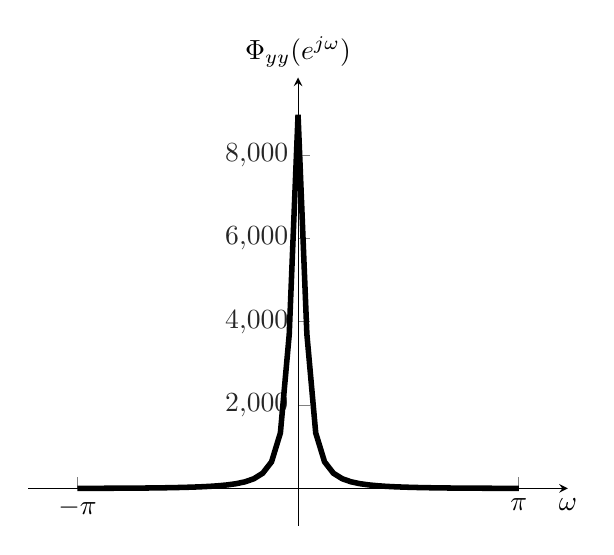
\begin{tikzpicture} 
		\begin{axis}[
		axis lines*=middle,
		enlargelimits = true,
		xmax=3.2,
		xmin=-3.2,
		ymin=0,
		axis line style={->,>=stealth},
		ylabel={$\Phi_{yy}(e^{j\omega})$},
		xlabel={$\omega$},
		every axis x label/.style={
			at={(ticklabel* cs:1)},
			anchor=north,
		},
		every axis y label/.style={
			at={(ticklabel* cs:1)},
			anchor=south,
		},
		xtick={-3.14, 3.14},
		xticklabels={$-\pi$, $\pi$},
		xticklabel style = {xshift=0cm},
		every outer y axis line/.append style={white!15!black},
		every y tick label/.append style={font=\color{white!15!black}},
		legend style={draw=white!15!black,fill=white,legend cell align=left}]
		\addplot[line width=2pt, domain=-pi:pi, samples=51] {10*(5+4*cos(deg(x)))/(1.81-1.8*cos(deg(x)))};
		\end{axis}
		\end{tikzpicture}
}
\end{center}

\subsection{(b)}

Following the hint, we rewrite \eqref{psd_yy} so that we can use the DTFT relation: 
\begin{equation}
e^{-a|n|} \longleftrightarrow \frac{1- e^{-2a}}{1+e^{-2a} -2e^{-a}\cos\omega}
\end{equation}

\begin{align} \nonumber
\Phi_{yy}(e^{j\omega}) &= \frac{50 + 40\cos(\omega)}{1.81 - 1.8\cos(\omega)} \\ \nonumber
&= \frac{50 + 40\cos(\omega)}{1.81 - 1.8\cos(\omega)}  + 40/1.8 - 40/1.8 \\ \nonumber
&= \frac{50 + 1.81\cdot 40/1.8}{1.81 - 1.8\cos(\omega)} - 40/1.8 \\ \nonumber
&= \frac{(50 + 1.81\cdot 40/1.8)}{1-0.81}\frac{1-0.81}{1 + 0.81 - 1.8\cos(\omega)} - 40/1.8 \\
&= 474.8538\frac{1-0.81}{1 + 0.81 - 1.8\cos(\omega)} - 22.2222
\end{align}

Now we can finally use the relation, for $a = -\ln(0.9) = 0.1054$. Hence, we can finally write:

\begin{equation}
\phi_{yy}[m] = 474.8538e^{-0.1054|n|} - 22.2222\delta[m]
\end{equation}

\subsection{(c)}
By definition,
\begin{equation}
\E(y^2[n]) = \phi_{yy}[0] = 452.6316
\end{equation}

\section{Problem 4}	
\subsection{(a)}
From the diagram $w[n] = x[n]\ast h_1[n]$. Therefore,
\begin{align}
\phi_{ww}[m] &= \phi_{xx}[m]\ast c_{h_1h_1}[m] = \phi_{xx}[m]\ast h_1[m]\ast h_1^*[-m]
\end{align}
\begin{align} \nonumber
\Phi_{ww}(e^{j\omega}) &= \Phi_{xx}(e^{j\omega})\cdot |H_1(e^{j\omega})|^2 \\
&= 10 \cdot |H_1(e^{j\omega})|^2
&= \begin{cases}
0, & |\omega| < \omega_c \\
10, & \omega_c < |\omega| < \pi
\end{cases}
\end{align}

\begin{center}
	\resizebox{0.5\linewidth}{!}{
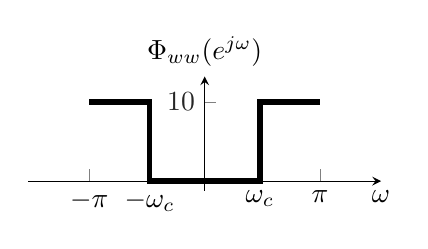
\begin{tikzpicture} 
	\begin{axis}[
	axis lines*=middle,
	enlargelimits = true,
	xmax=4,
	xmin=-4,
	ymin=0,
	ymax=12,
	width=0.5\textwidth,
	height=0.25\textwidth,
	axis line style={->,>=stealth},
	ylabel={$\Phi_{ww}(e^{j\omega})$},
	xlabel={$\omega$},
	every axis x label/.style={
		at={(ticklabel* cs:1)},
		anchor=north,
	},
	every axis y label/.style={
		at={(ticklabel* cs:1)},
		anchor=south,
	},
	xtick={-3.14, -1.5, 0, 1.5, 3.14},
	ytick={10},
	xticklabels={$-\pi$, $-\omega_c$, $0$, $\omega_c$, $\pi$},
	xticklabel style = {xshift=0cm},
	every outer y axis line/.append style={white!15!black},
	every y tick label/.append style={font=\color{white!15!black}},
	legend style={draw=white!15!black,fill=white,legend cell align=left}]
	\addplot[line width=2pt] coordinates {(-pi, 10) (-1.5, 10) (-1.5, 0) (1.5, 0) (1.5, 10) (pi, 10)};
	\end{axis}
\end{tikzpicture}
}
\end{center}

\subsection{(b)}

By inspection, we can write the PSD of $w$ as a constant minus the ideal lowpass filter from $-\omega_c$ to $\omega_c$. The inverse DTFT of a constant is an impulse at the origin, and the inverse DTFT of the ideal lowpass filter is a sinc function.

\begin{equation}
\phi_{ww}[m] = 10\delta[m] - 10\frac{\sin\omega_cm}{\pi m}
\end{equation}
	
\subsection{(c)}
\begin{equation}
\E(w^2[n]) = \phi_{ww}[0] = 10 - 10\frac{\omega_c}{\pi} = 10(1 - \frac{\omega_c}{\pi})
\end{equation}
	
\subsection{(d)}

For system 2 we have
\begin{equation}
h_2[m] = \delta[m-5] \longleftrightarrow H_2(e^{j\omega}) = e^{-j5\omega}.
\end{equation}

Therefore,
\begin{equation}
\Phi_{yy}(e^{j\omega}) = \Phi_{ww}(e^{j\omega})|H_2(e^{j\omega})|^2 = \Phi_{ww}(e^{j\omega})
\end{equation}
Consequently, $\phi_{yy}[m] = \phi_{ww}[m]$.

\begin{equation}
\E(y^2[n]) = \phi_{yy}[0] =  \phi_{ww}[0] = 10(1 - \frac{\omega_c}{\pi})
\end{equation}

\subsection{(e)}
\begin{align}\nonumber
\phi_{wy}[m] &= \E(w[n]y[n+m]) \\ 
&= \E(w[n]w[n+m-5]) \\ \nonumber
&= \phi_{ww}[m-5] \\
&=\begin{cases}
10(1-\frac{\omega_c}{\pi}), & m = 5 \\
-10\frac{\sin\omega_c(m-5)}{\pi(m-5)}, & m \neq 5 \\
\end{cases}
\end{align}
	
\section{Problem 5}
\subsection{(a)}

\begin{center}
	\resizebox{0.5\linewidth}{!}{\begin{tikzpicture}
\begin{axis}[
	name=plot1,
	axis lines*=middle,
	enlargelimits = false,
	clip=false,
	scale only axis,
	width=0.5\textwidth,
	height=0.15\textwidth,
	ymin=0,
	ymax=1,
	xmin=-5,
	xmax=5,
	axis line style={->,>=stealth},
	xlabel={\small $x$},
	ylabel={\small $p_x(x)$},
	every axis x label/.style={
		at={(ticklabel* cs:1)},
		%xshift=0.2cm,
		anchor=north,
	},
	every axis y label/.style={
		at={(ticklabel* cs:1)},
		anchor=south,
	},
	ytick={0.5},
	xtick={-1, 1},
	every outer y axis line/.append style={white!15!black},
	every y tick label/.append style={font=\color{white!15!black}},
	legend style={draw=white!15!black,fill=white,legend cell align=left}]
	\addplot[ycomb, mark=*, fill=white, mark options={scale=0.75, fill=white}, line width=1pt, domain=0:3, samples=4] coordinates {(-1, 0.5) (1, 0.5)};
\end{axis}
\begin{axis}[
	name=plot2,
	at=(plot1.below south east), anchor=above north east,
	axis lines*=middle,
	enlargelimits = false,
	clip=false,
	scale only axis,
	width=0.5\textwidth,
	height=0.14\textwidth,
	ymin=0,
	ymax=2,
	xmin=-5,
	xmax=5,
	axis line style={->,>=stealth},
	xlabel={\small $m$},
	ylabel={\small $\phi_{xx}[m] = \delta[m]$},
	yticklabel style = {yshift=0cm},
	every axis x label/.style={
		at={(ticklabel* cs:1)},
		%xshift=0.2cm,
		anchor=north,
	},
	every axis y label/.style={
		at={(ticklabel* cs:0.8)},
		anchor=south,
	},
	ytick={1},
	xtick=\empty,
	every outer y axis line/.append style={white!15!black},
	every y tick label/.append style={font=\color{white!15!black}},
	legend style={draw=white!15!black,fill=white,legend cell align=left}]
	\addplot[ycomb, mark=*, fill=white, mark options={scale=0.75, fill=white}, line width=1pt, domain=-5:5, samples=11] {x==0};
\end{axis}
\begin{axis}[
	name=plot3,
	at=(plot2.below south east), anchor=above north east,
	axis lines*=middle,
	enlargelimits = false,
	clip=false,
	scale only axis,
	width=0.5\textwidth,
	height=0.14\textwidth,
	ymin=0,
	ymax=2,
	xmin=-5,
	xmax=5,
	axis line style={->,>=stealth},
	xlabel={$\omega$},
	yticklabel style = {yshift=0.2cm},
	ylabel={$\Phi_{xx}(e^{j\omega}) = 1$},
	every axis x label/.style={
		at={(ticklabel* cs:1)},
		%xshift=0.2cm,
		anchor=north,
	},
	every axis y label/.style={
		at={(ticklabel* cs:1)},
		anchor=south,
		xshift=0cm,
	},
	ytick={1},
	xtick={-3.14, 3.14},
	xticklabels={$-\pi$, $\pi$},
	every outer y axis line/.append style={white!15!black},
	every y tick label/.append style={font=\color{white!15!black}},
	legend style={draw=white!15!black,fill=white,legend cell align=left}]
	\addplot[line width=1pt, domain=-3.14:3.14, samples=2] {1};
\end{axis}
\end{tikzpicture}
}
\end{center}

\subsection{(b)}
\begin{align} \nonumber
\phi_{yy}[m] &= \E(y[m]y[n+m]) \\ \nonumber
&=\frac{1}{L^2}\sum_{k=0}^{L-1}\sum_{l=0}^{L-1} \E(x[n-k]y[n+m-l]) \\ \nonumber
&=\frac{1}{L^2}\sum_{k=0}^{L-1}\sum_{l=0}^{L-1} \phi_{xx}[m+k-l] \\
&=\frac{1}{L^2}\sum_{\substack{ 0\leq k \leq L-1 \\ 0\leq l\leq L-1 \\ l-k=m}} 1 = \begin{cases}
	\frac{L-|m|}{L^2}, & |m|<L \\
	0, & \text{otherwise}
\end{cases}
\end{align}

For $L = 4$, 
\begin{center}
	\resizebox{0.5\linewidth}{!}{
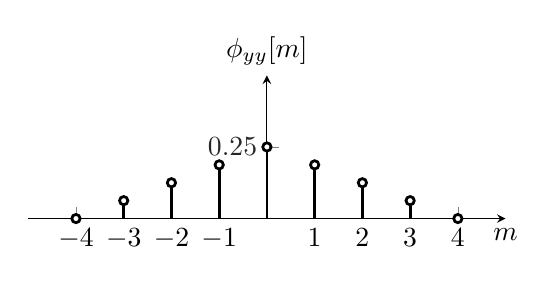
\begin{tikzpicture}
	\begin{axis}[
		axis lines*=middle,
		enlargelimits = false,
		clip=false,
		scale only axis,
		width=0.5\textwidth,
		height=0.15\textwidth,
		ymin=0,
		ymax=0.5,
		xmin=-5,
		xmax=5,
		axis line style={->,>=stealth},
		xlabel={$m$},
		ylabel={$\phi_{yy}[m]$},
		every axis x label/.style={
			at={(ticklabel* cs:1)},
			anchor=north,
		},
		every axis y label/.style={
			at={(ticklabel* cs:1)},
			anchor=south,
		},
		ytick={0.25},
		xtick={-4,...,4},
		every outer y axis line/.append style={white!15!black},
		every y tick label/.append style={font=\color{white!15!black}},
		legend style={draw=white!15!black,fill=white,legend cell align=left}]
		\addplot[ycomb, mark=*, fill=white, mark options={scale=0.75, fill=white}, line width=1pt, domain=0:3, samples=4] coordinates {(-4, 0) (-3, 1/16) (-2, 1/8) (-1, 3/16) (0, 1/4) (4, 0) (3, 1/16) (2, 1/8) (1, 3/16)};
	\end{axis}
\end{tikzpicture}
}
\end{center}

\subsection{(c)}
For the mean of $y[m]$:
\begin{align} \nonumber
\mu_y &= \E(y[m]) = \E\bigg(\frac{1}{L}\sum_{k=0}^{L-1}x[m-k]\bigg) \\ \nonumber
&=\frac{1}{L}\sum_{k=0}^{L-1}\E(x[m-k])
&=0
\end{align}

For the average power of $y[m]$:
\begin{align} \nonumber
\E(y^2[m]) = \phi_{yy}[0] = \frac{1}{L}
\end{align}

\subsection{(d)}
By inspecting all combinations of inputs patterns:

\begin{center}
	\begin{tabular}{l|c|c}
	Input patterns & $y$ & $p_y(y)$ \\
	\hline
	($-1, -1, -1, -1$) & $-1$ & $1/16$ \\
	Permutations of ($-1, -1, -1, 1$) & $-1/2$ & $1/4$ \\
	Permutations of ($-1, -1, 1, 1$) & $0$ & $3/8$ \\
	Permutations of ($-1, 1, 1, 1$) & $1/2$ & $1/4$ \\	
	($1, 1, 1, 1$) & $1$ & $1/16$ \\
	\hline
\end{tabular}
\end{center}

\begin{center}
	\resizebox{0.5\linewidth}{!}{
		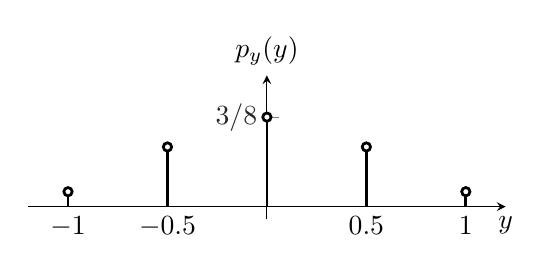
\begin{tikzpicture}
		\begin{axis}[
		axis lines*=middle,
		enlargelimits = true,
		clip=false,
		scale only axis,
		width=0.5\textwidth,
		height=0.15\textwidth,
		ymin=0,
		ymax=0.5,
		xmin=-1,
		xmax=1,
		axis line style={->,>=stealth},
		xlabel={$y$},
		ylabel={$p_y(y)$},
		every axis x label/.style={
			at={(ticklabel* cs:1)},
			anchor=north,
		},
		every axis y label/.style={
			at={(ticklabel* cs:1)},
			anchor=south,
		},
		ytick={0.375},
		yticklabels={$3/8$},
		xtick={-1, -0.5, 0, 0.5, 1},
		every outer y axis line/.append style={white!15!black},
		every y tick label/.append style={font=\color{white!15!black}},
		legend style={draw=white!15!black,fill=white,legend cell align=left}]
		\addplot[ycomb, mark=*, fill=white, mark options={scale=0.75, fill=white}, line width=1pt] coordinates {(-1, 1/16) (-1/2, 1/4) (0, 3/8) (1, 1/16) (1/2, 1/4)};
		\end{axis}
		\end{tikzpicture}
}
\end{center}

\subsection{(e)}

The convolutions are discrete because $x$ is a discrete random variable, and therefore its probability mass function $p_x(x)$ is a discrete function of $x$.

\begin{center}
	\begin{tabular}{c|c|c}
	$L$ & Possible $y[m]$  values & Corresponding probabilities \\
	\hline
	2 & $-1, 0, 1$ & $1/4, 1/2, 1/4$ \\
	3 & $-1, -1/3, 1/3, 1$ & $1/8, 3/8, 3/8, 1/8$ \\
	4 & $-1, -1/2, 0, 1/2, 1$ & $1/16, 1/4, 3/8, 1/4, 1/16$ \\
	5 & $-1, -3/5, -1/5, 1/5, 3/5, 1$ &  $1/32, 5/32, 5/16, 5/16, 5/32, 1/32$\\
	\hline
\end{tabular}
\end{center}

If the system were an $L$-point running sum, the possible values of $y[m]$ would be scaled by $m$, but the corresponding probabilities would not change.
\begin{center}
	\begin{tabular}{c|c|c}
		$L$ & Possible $y[m]$ values & Corresponding probabilities \\
		\hline
		2 & $-2, 0, 2$ & $1/4, 1/2, 1/4$ \\
		3 & $-3, -1, 1, 3$ & $1/8, 3/8, 3/8, 1/8$ \\
		4 & $-4, -2, 0, 2, 4$ & $1/16, 1/4, 3/8, 1/4, 1/16$ \\
		5 & $-5, -3, -1, 1, 3, 5$ &  $1/32, 5/32, 5/16, 5/16, 5/32, 1/32$ \\
		\hline
	\end{tabular}
\end{center}

\subsection{(f)}

\FloatBarrier
\begin{figure}[ht]
\centering
\includegraphics[scale=0.7]{q16f.eps}
\caption{$p_y(y)$ for $L = 5$ (left) and for $L = 6$ (right).}
\end{figure}
\FloatBarrier

\textbf{Code:}
% This file was automatically created from the m-file 
% "m2tex.m" written by USL. 
% The fontencoding in this file is UTF-8. 
%  
% You will need to include the following two packages in 
% your LaTeX-Main-File. 
%  
% \usepackage{color} 
% \usepackage{fancyvrb} 
%  
% It is advised to use the following option for Inputenc 
% \usepackage[utf8]{inputenc} 
%  
%% Insert these lines where you wish to break line 
% \end{tabular} 
% \newpage 
% \begin{tabular}{|p{\textwidth}|} 
  
% definition of matlab colors: 
\definecolor{mblue}{rgb}{0,0,1} 
\definecolor{mgreen}{rgb}{0.13333,0.5451,0.13333} 
\definecolor{mred}{rgb}{0.62745,0.12549,0.94118} % change to {0,0,0} in case of bug 
\definecolor{mgrey}{rgb}{0.5,0.5,0.5} 
\definecolor{mdarkgrey}{rgb}{0.25,0.25,0.25} 
  
\DefineShortVerb[fontfamily=courier,fontseries=m]{\$} 
\DefineShortVerb[fontfamily=courier,fontseries=b]{\#} 
\begin{tabular}{|p{\textwidth}|} 
\hline 
  
\noindent          
 \hspace*{-1.6em}{\scriptsize 1}$  $\color{mblue}$function$\color{black}$ [p, x] = out_prob(L)$\\
 \hspace*{-1.6em}{\scriptsize 2}$  $\\
 \hspace*{-1.6em}{\scriptsize 3}$  p2 = [1 1]/2; $\color{mgreen}$% pmf for L = 1$\color{black}$$\\
 \hspace*{-1.6em}{\scriptsize 4}$  p = p2;$\\
 \hspace*{-1.6em}{\scriptsize 5}$  $\color{mblue}$for$\color{black}$ k = 1:L-1$\\
 \hspace*{-1.6em}{\scriptsize 6}$      p = conv(p, p2);$\\
 \hspace*{-1.6em}{\scriptsize 7}$  $\color{mblue}$end$\color{black}$$\\
 \hspace*{-1.6em}{\scriptsize 8}$  $\\
 \hspace*{-1.6em}{\scriptsize 9}$  $\color{mgreen}$% since x takes on equally spaced values between -1 and 1$\color{black}$$\\
 \hspace*{-2em}{\scriptsize 10}$  x = linspace(-1,1, length(p)); $\\ 
  
\hline 
\end{tabular} 
\UndefineShortVerb{\$} 
\UndefineShortVerb{\#}

\subsection{(g)}
\begin{align} \nonumber
\Phi_{yy}(e^{j\omega}) &= \Phi_{xx}(e^{j\omega})|H(e^{j\omega})|^2 \\ \nonumber
& =\frac{1}{L^2}|\bigg|\frac{1-e^{-j\omega L}}{1-e^{-j\omega}}\bigg|^2 \\ \nonumber
& =\frac{1}{L^2}\bigg(\frac{1-e^{-j\omega  L}}{1-e^{-j\omega}}\bigg)\bigg(\frac{1-e^{j\omega L}}{1-e^{j\omega}}\bigg) \\
&= \frac{1}{L^2}\bigg(\frac{1-\cos(\omega L)}{1 - \cos(\omega)}\bigg)
\end{align}

\FloatBarrier
\begin{figure}[ht]
\centering
\includegraphics[scale=0.7]{q16g.eps}
\caption{Power spectrum density of the output of a 4-point moving average filter.}
\label{fig:q16f}
\end{figure}
\FloatBarrier

\subsection{(h)}

The possible values of the output would remain the same, but the probability mass function of the output would not be symmetric. Autocorrelation function and the power spectrum density do not depend on the input distribution, as long as the input remains uncorrelated. 

\end{document}
